\documentclass[11pt]{article}
\usepackage[textwidth=18.0cm, textheight=23.0cm, top=2.0cm]{geometry}
\usepackage{pst-all}
\usepackage{amssymb}
\usepackage{tikz}
\usepackage{underscore}\begin{document}
\pagestyle{empty}


ClassName: \underline{\textbf{Class_10.2bp-4}}
\par
BinSize: \underline{\textbf{100 × 100}}
\par
ReduceSize: \underline{\textbf{100 × 100}}
\par
TypeNum: \underline{\textbf{20}}
\par
Num: \underline{\textbf{20}}
\par
OutS: \underline{\textbf{40000}}
\par
InS: \underline{\textbf{31540}}
\par
Rate: \underline{\textbf{0.789}}
\par
UB: \underline{\textbf{4}}
\par
LB0: \underline{\textbf{4}}
\par
LB: \underline{\textbf{4}}
\par
LBWithCut: \underline{\textbf{4}}
\par
NodeCut: \underline{\textbf{0}}
\par
ExtendedNodeCnt: \underline{\textbf{1}}
\par
GenNodeCnt: \underline{\textbf{1}}
\par
PrimalNode: \underline{\textbf{0}}
\par
ColumnCount: \underline{\textbf{4}}
\par
TotalCutCount: \underline{\textbf{0}}
\par
RootCutCount: \underline{\textbf{0}}
\par
LPSolverCnt: \underline{\textbf{1}}
\par
PricingSolverCnt: \underline{\textbf{0}}
\par
BranchAndBoundNum: \underline{\textbf{1}}
\par
isOpt: \underline{\textbf{true}}
\par
TimeOnInitSolution: \underline{\textbf{600.000 s}}
\par
TimeOnPrimal: \underline{\textbf{0.000 s}}
\par
TimeOnPricing: \underline{\textbf{0.000 s}}
\par
TimeOnRmp: \underline{\textbf{0.047 s}}
\par
TotalTime: \underline{\textbf{600.313 s}}
\par
\newpage


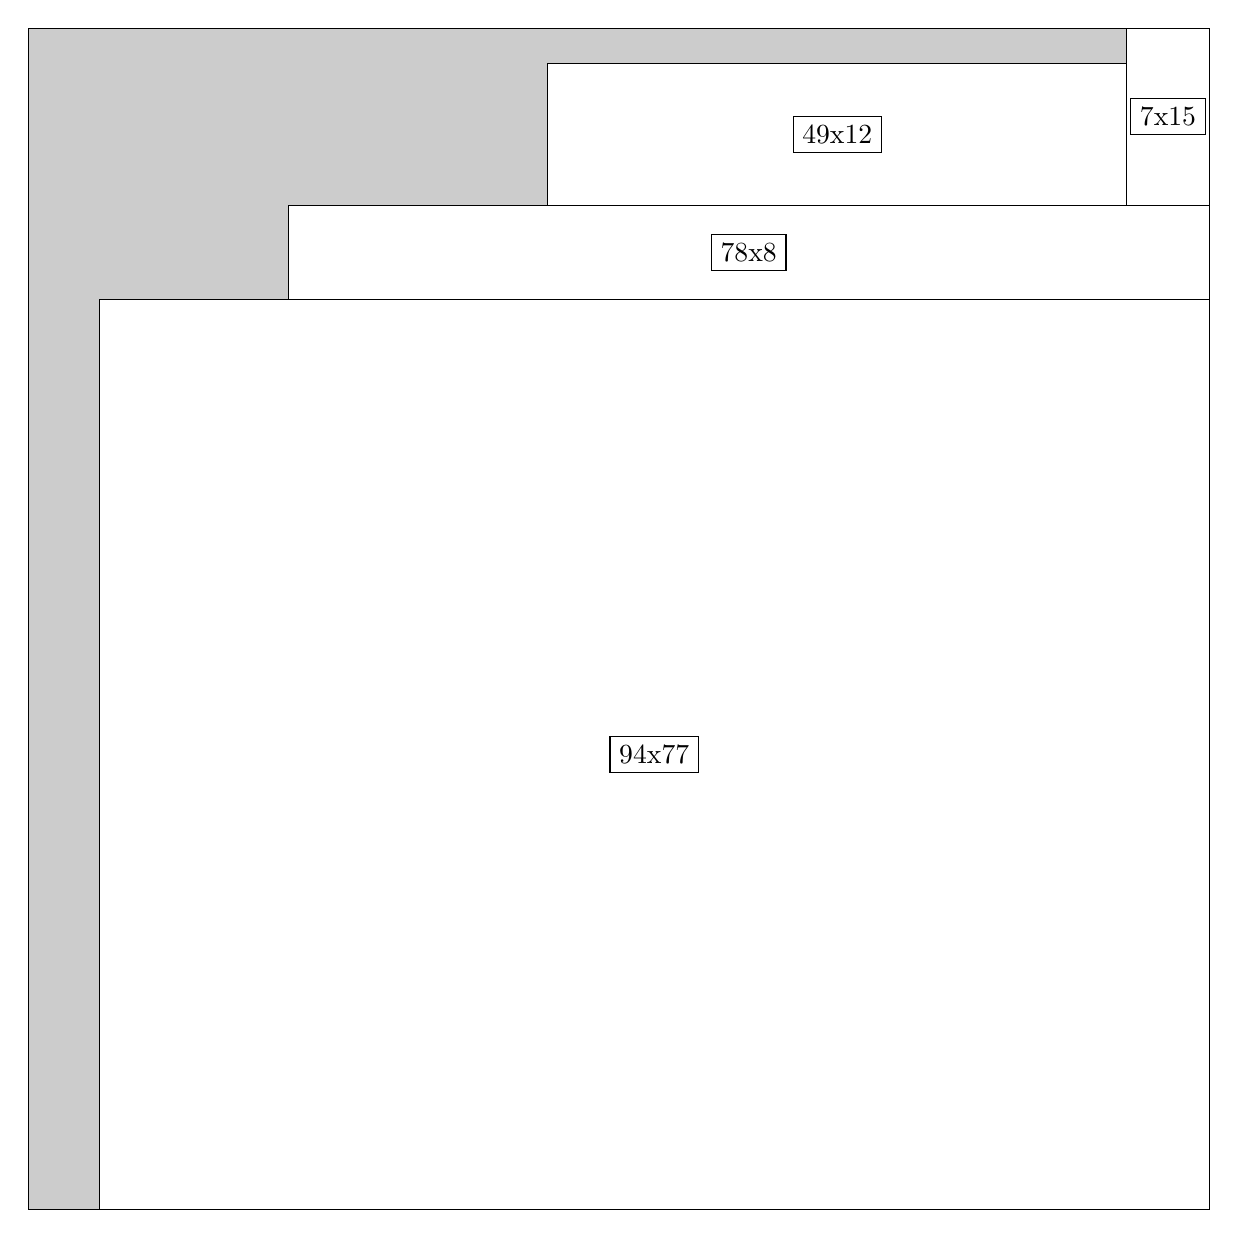
\begin{tikzpicture}[shorten >=1pt,scale=1.0,every node/.style={scale=1.0},->]
\tikzstyle{vertex}=[circle,fill=black!25,minimum size=14pt,inner sep=0pt]
\filldraw[fill=gray!40!white, draw=black] (0,0) rectangle (15.0,15.0);
\foreach \name/\x/\y/\w/\h in {94x77/0.8999999999999999/0.0/14.1/11.549999999999999,78x8/3.3/11.549999999999999/11.7/1.2,7x15/13.95/12.75/1.05/2.25,49x12/6.6/12.75/7.35/1.7999999999999998}
\filldraw[fill=white!40!white, draw=black] (\x,\y) rectangle node[draw] (\name) {\name} ++(\w,\h);
\end{tikzpicture}


w =94 , h =77 , x =6 , y =0 , v =7238
\par
w =78 , h =8 , x =22 , y =77 , v =624
\par
w =7 , h =15 , x =93 , y =85 , v =105
\par
w =49 , h =12 , x =44 , y =85 , v =588
\par
\newpage


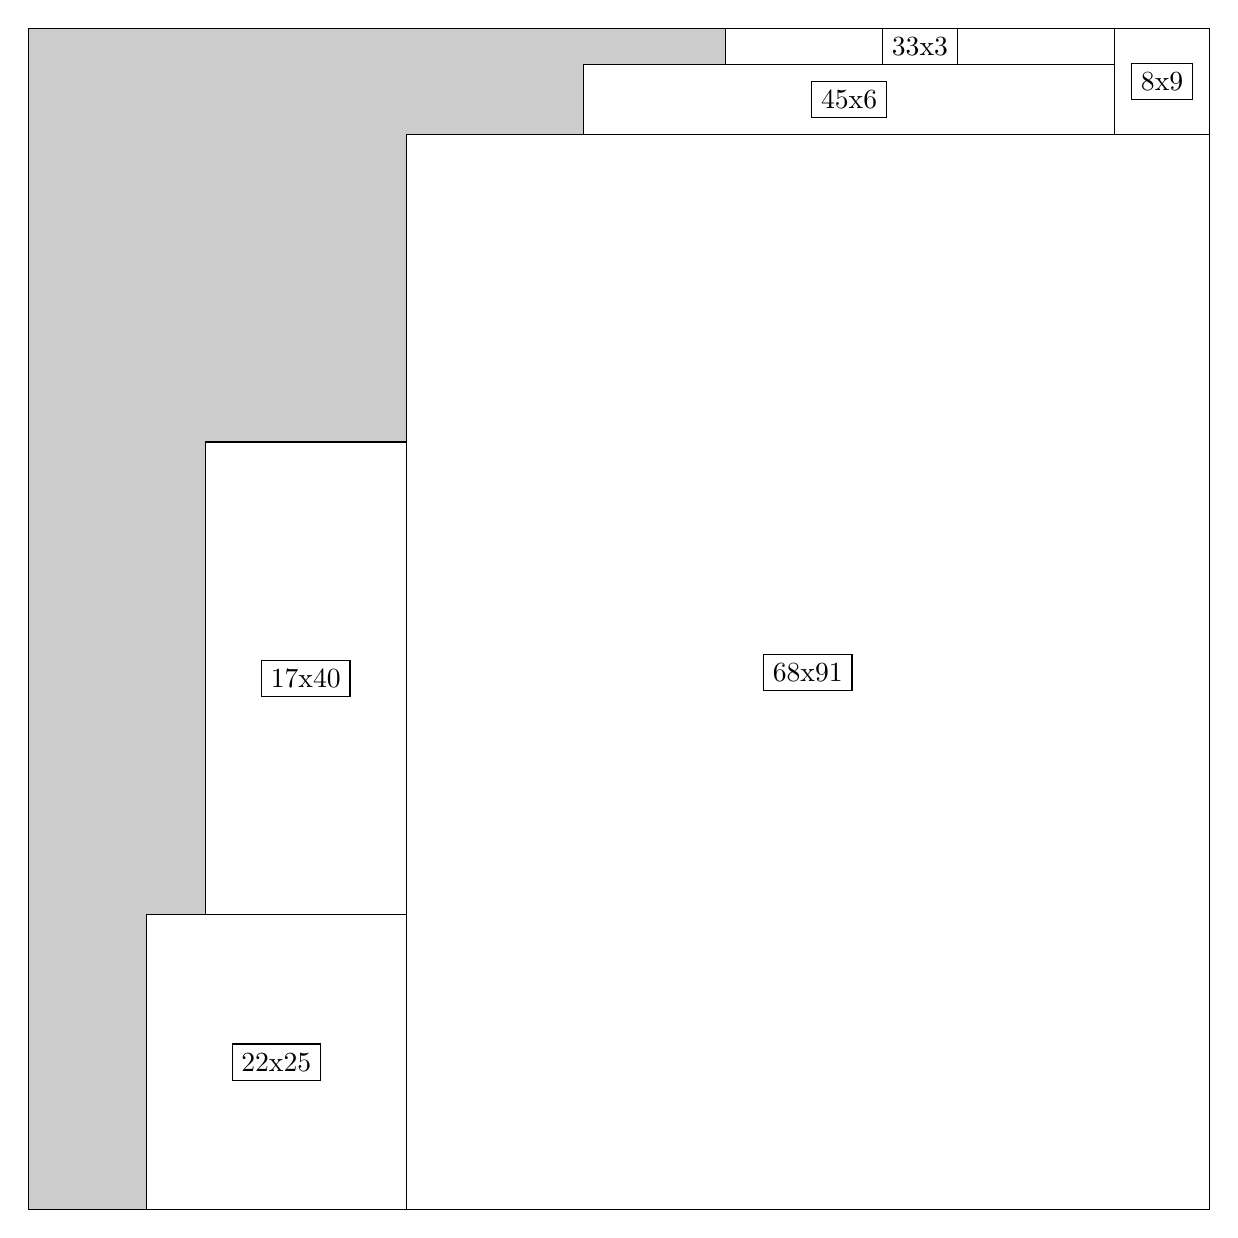
\begin{tikzpicture}[shorten >=1pt,scale=1.0,every node/.style={scale=1.0},->]
\tikzstyle{vertex}=[circle,fill=black!25,minimum size=14pt,inner sep=0pt]
\filldraw[fill=gray!40!white, draw=black] (0,0) rectangle (15.0,15.0);
\foreach \name/\x/\y/\w/\h in {68x91/4.8/0.0/10.2/13.65,8x9/13.799999999999999/13.65/1.2/1.3499999999999999,45x6/7.05/13.65/6.75/0.8999999999999999,33x3/8.85/14.549999999999999/4.95/0.44999999999999996,22x25/1.5/0.0/3.3/3.75,17x40/2.25/3.75/2.55/6.0}
\filldraw[fill=white!40!white, draw=black] (\x,\y) rectangle node[draw] (\name) {\name} ++(\w,\h);
\end{tikzpicture}


w =68 , h =91 , x =32 , y =0 , v =6188
\par
w =8 , h =9 , x =92 , y =91 , v =72
\par
w =45 , h =6 , x =47 , y =91 , v =270
\par
w =33 , h =3 , x =59 , y =97 , v =99
\par
w =22 , h =25 , x =10 , y =0 , v =550
\par
w =17 , h =40 , x =15 , y =25 , v =680
\par
\newpage


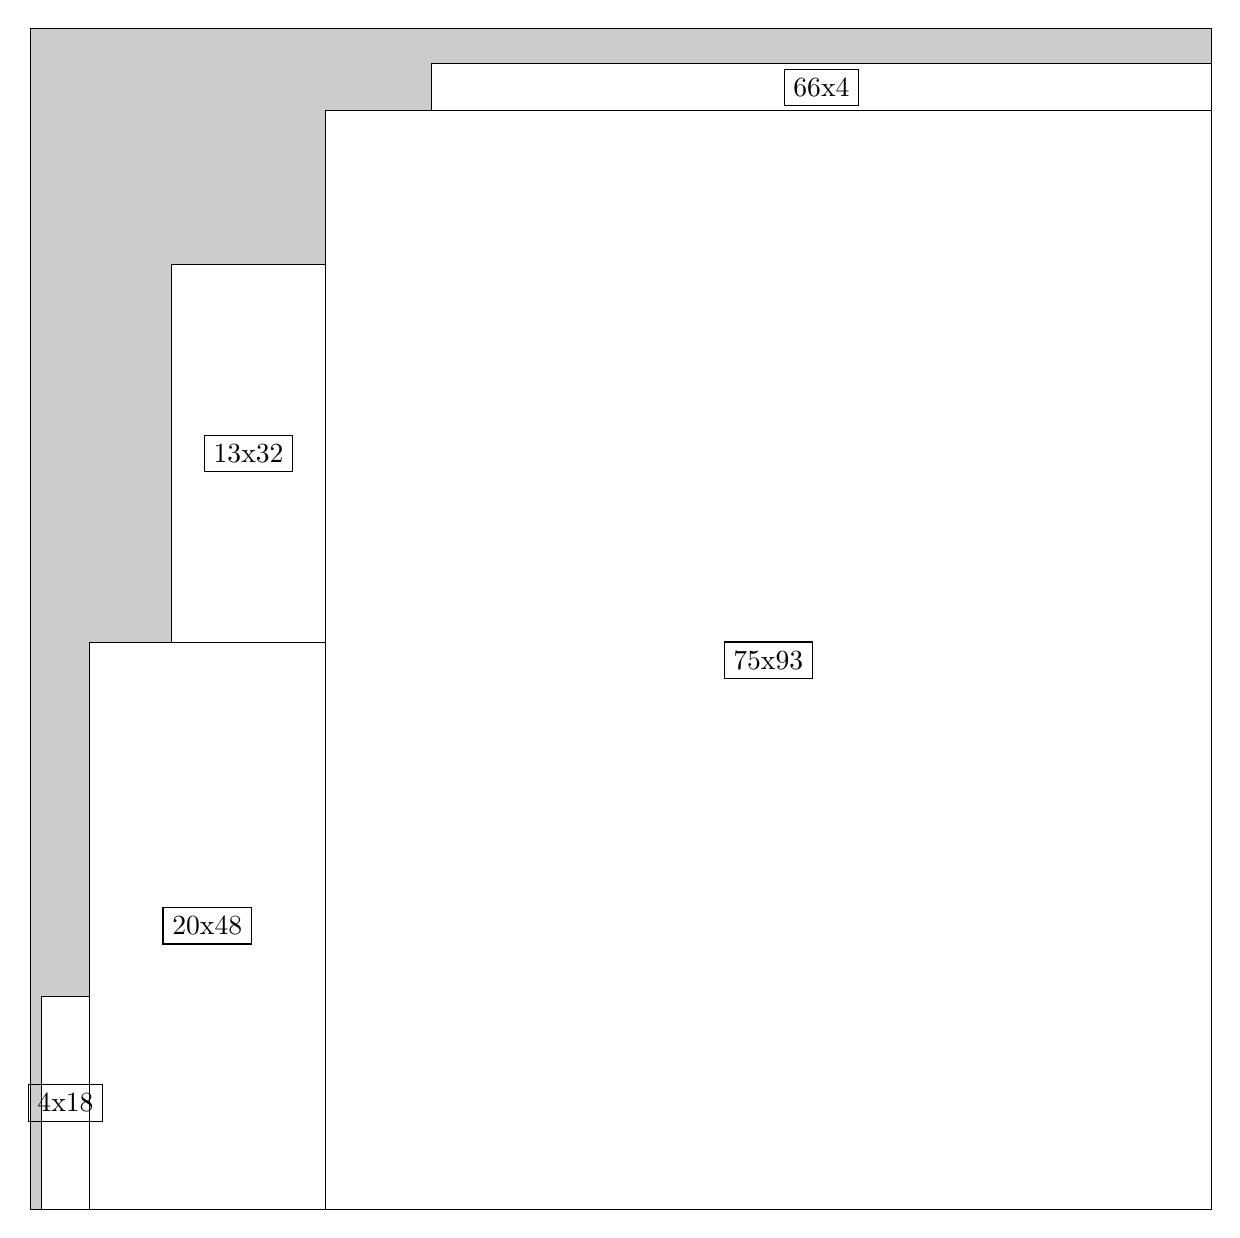
\begin{tikzpicture}[shorten >=1pt,scale=1.0,every node/.style={scale=1.0},->]
\tikzstyle{vertex}=[circle,fill=black!25,minimum size=14pt,inner sep=0pt]
\filldraw[fill=gray!40!white, draw=black] (0,0) rectangle (15.0,15.0);
\foreach \name/\x/\y/\w/\h in {75x93/3.75/0.0/11.25/13.95,20x48/0.75/0.0/3.0/7.199999999999999,4x18/0.15/0.0/0.6/2.6999999999999997,13x32/1.7999999999999998/7.199999999999999/1.95/4.8,66x4/5.1/13.95/9.9/0.6}
\filldraw[fill=white!40!white, draw=black] (\x,\y) rectangle node[draw] (\name) {\name} ++(\w,\h);
\end{tikzpicture}


w =75 , h =93 , x =25 , y =0 , v =6975
\par
w =20 , h =48 , x =5 , y =0 , v =960
\par
w =4 , h =18 , x =1 , y =0 , v =72
\par
w =13 , h =32 , x =12 , y =48 , v =416
\par
w =66 , h =4 , x =34 , y =93 , v =264
\par
\newpage


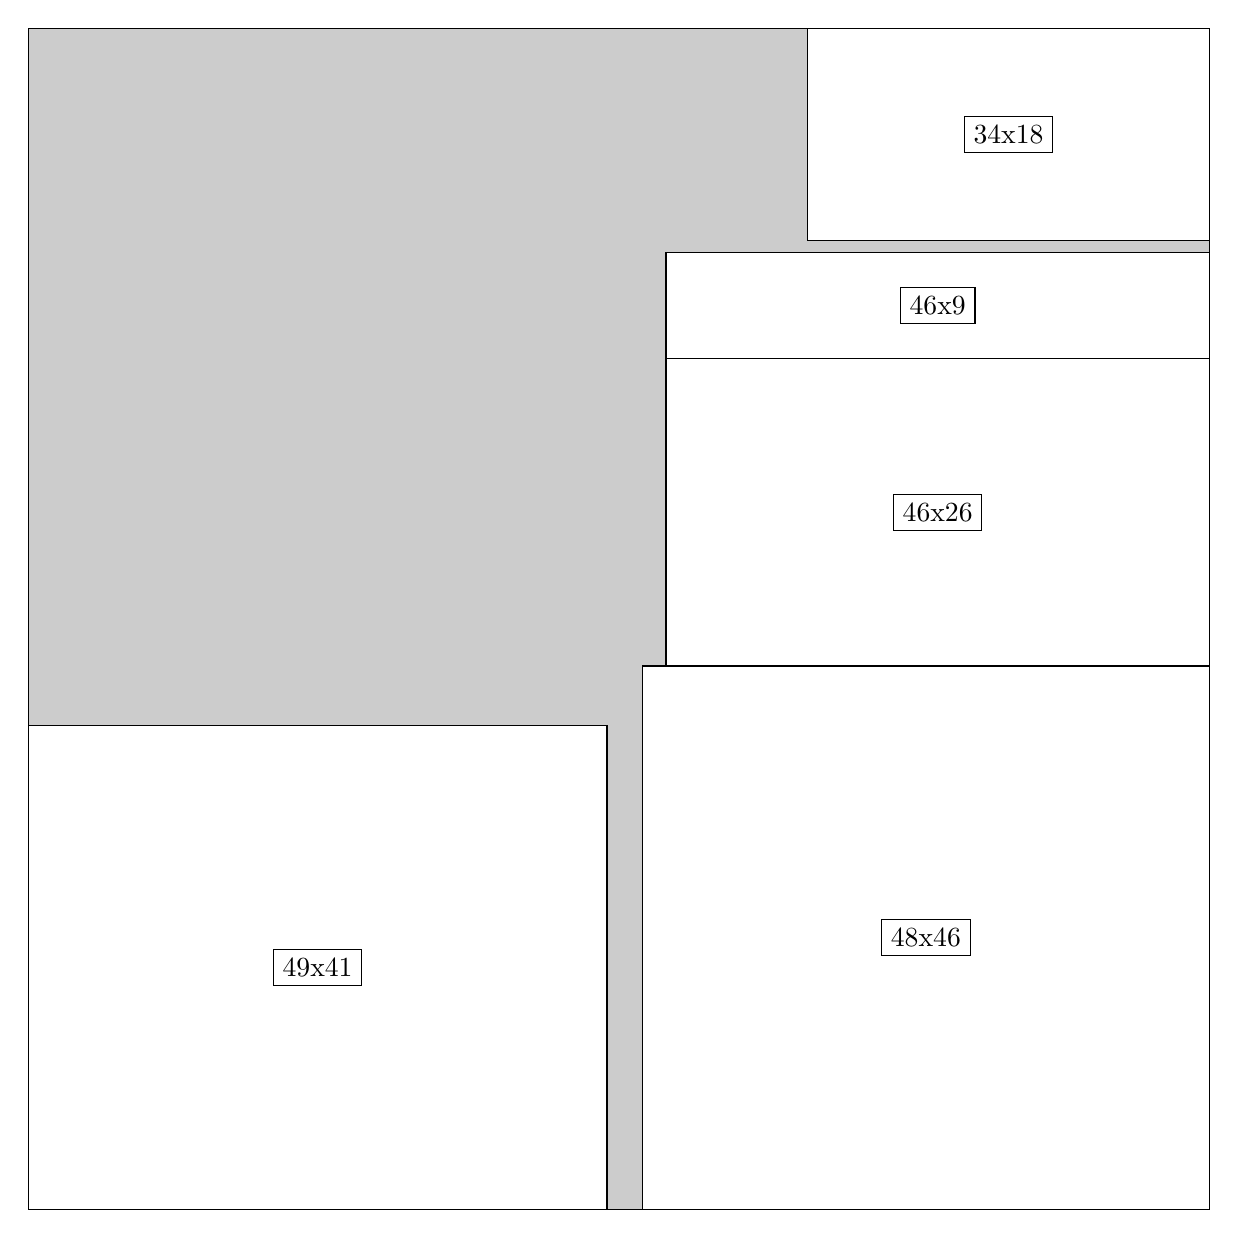
\begin{tikzpicture}[shorten >=1pt,scale=1.0,every node/.style={scale=1.0},->]
\tikzstyle{vertex}=[circle,fill=black!25,minimum size=14pt,inner sep=0pt]
\filldraw[fill=gray!40!white, draw=black] (0,0) rectangle (15.0,15.0);
\foreach \name/\x/\y/\w/\h in {48x46/7.8/0.0/7.199999999999999/6.8999999999999995,46x26/8.1/6.8999999999999995/6.8999999999999995/3.9,46x9/8.1/10.799999999999999/6.8999999999999995/1.3499999999999999,49x41/0.0/0.0/7.35/6.1499999999999995,34x18/9.9/12.299999999999999/5.1/2.6999999999999997}
\filldraw[fill=white!40!white, draw=black] (\x,\y) rectangle node[draw] (\name) {\name} ++(\w,\h);
\end{tikzpicture}


w =48 , h =46 , x =52 , y =0 , v =2208
\par
w =46 , h =26 , x =54 , y =46 , v =1196
\par
w =46 , h =9 , x =54 , y =72 , v =414
\par
w =49 , h =41 , x =0 , y =0 , v =2009
\par
w =34 , h =18 , x =66 , y =82 , v =612
\par
\newpage


\end{document}